\documentclass[12pt, titlepage]{article}
% naglowek i stopka
\usepackage{fancyhdr}
% polskie znaki
\usepackage[utf8]{inputenc}
\usepackage[polish]{babel}
\usepackage{polski}
% czcionka Times
\usepackage[T1]{fontenc}
\usepackage{mathptmx}
% ------------------
% marginesy
\usepackage{geometry} 
\newgeometry{tmargin=3cm, bmargin=3cm, lmargin=2cm, rmargin=2cm}
% przedefiniowanie kolumn w tabelach
% mozna ustawiac im szerokosc
\usepackage{array}
\newcolumntype{L}[1]{>{\raggedright\let\newline\\\arraybackslash\hspace{0pt}}m{#1}}
\newcolumntype{C}[1]{>{\centering\let\newline\\\arraybackslash\hspace{0pt}}m{#1}}
\newcolumntype{R}[1]{>{\raggedleft\let\newline\\\arraybackslash\hspace{0pt}}m{#1}}
\newcolumntype{N}{@{}m{0pt}@{}}
% ------------------------------
% napisy nad tabelami
\usepackage[font=small,format=plain,up,textfont=normal,up,justification=justified,singlelinecheck=false]{caption}
% tabele na kilka stron
\usepackage{longtable}
% ustawienie tabeli w miejscu
\usepackage{float}
% spis tresci z linkami do sekcji
\usepackage{hyperref}
\hypersetup{
	colorlinks,
	citecolor=black,
	filecolor=black,
	linkcolor=black,
	urlcolor=blue
}
% kolowanie tabeli
\usepackage[table]{xcolor}
% dodawanie obrazkow
\usepackage{graphicx}

\fancypagestyle{firstpage}{					% strona tytulowa
	\renewcommand{\headrulewidth}{0pt}
	\renewcommand{\footrulewidth}{0.4pt}
	\fancyhf{}% clear all fields
	\fancyfoot[C]{Poznań, \today}%
	\fancyhead[C]
		{
		POLITECHNIKA POZNAŃSKA\\
		WYDZIAŁ ELEKTRYCZNY, INFORMATYKA\\
		SEMESTR VI, GRUPA BSI-2
		}
}

\fancypagestyle{plain}{						% zwykla strona
	\renewcommand{\headrulewidth}{0pt}%
	\fancyhf{}% clear all fields
	\fancyfoot[R]{\thepage}%
}
\pagestyle{plain}


\begin{document}
	\begin{titlepage}
		\thispagestyle{firstpage}
		\centering
			\vspace*{5cm}
			{\huge Podstawy Teleinformatyki\\
				WebScrapper / Metawyszukiwarka\\}
			\vspace{6cm}
			{\large \url{https://github.com/vizarch/projektPT}\\}
			\vspace{1cm}
			{\large
			Paweł Soja\\
			Numer indeksu: 122031\\
			pawel.soja@student.put.poznan.pl\\
			\vspace{0.5cm}
			Krzysztof Łuczak\\
			Numer indeksu: 122008\\
			krzysztof.t.luczak@student.put.poznan.pl\\
			\vspace{0.5cm}
			Dawid Wiktorski\\
			Numer indeksu: 122056\\
			dawid.wiktorski@student.put.poznan.pl\\}
	\end{titlepage}
	\tableofcontents
	\listoftables
	
	\newpage
	\section{Opis i uzasadnienie wyboru tematu}
	Celem projektu jest zaprojektowanie i zbudowanie platformy do zbierania i prezentowania danych z różnych stron internetowych. Platforma składa się z serwisu internetowego prezentującego dane użytkownikom zalogowanym oraz z aplikacji zbierających te dane.
	
	Temat wybraliśmy, ponieważ interesuje nas dziedzina przetwarzania danych. Chcielibyśmy poznać technologie scrapingu, parsowania stron internetowych oraz język Python, framework Django i technologie front-endowe tj. HTML5, Javascript. Jednocześnie nie znaleźliśmy zadowalającego nas serwisu, który udostępniałby takie usługi, dlatego sami zdecydowaliśmy zrobić swój.
	\section{Podział prac pomiędzy członków zespołu}
	{\setlength{\arrayrulewidth}{1mm}
	\setlength{\tabcolsep}{10pt}
	\renewcommand{\arraystretch}{2.5}
	{\rowcolors{1}{green!80!yellow!50}{green!70!yellow!40}
	\begin{table}[H]
		\centering
		\caption{Podział prac}
		\label{podzial_prac}
		\begin{tabular}{  C{2cm} | C{6cm} | C{8cm} | @{}m{0pt}@{}}
												% ostatnie krzaki to wysokosc wiersza
			\hline % ostatnia pusta kolumna to trik -> zle wyrownanie ostatniej kolumny
			\textbf{Lp.} &	\textbf{Opis} &	\textbf{Osoby} &\\[0.5cm]
			\hline
			1.	&	Baza danych			&	Wszyscy &\\[0.5cm] 
			\hline
			2.	&	Projekt interfejsu	&	Paweł Soja &\\[0.5cm]
			\hline
			3.	&	Front-end serwisu	&	Paweł Soja &\\[0.5cm]
			\hline
			4.	&	Back-end serwisu	&	Krzysztof Łuczak, Dawid Wiktorski &\\[0.5cm]
			\hline
			5.	&	Moduł I				&	Paweł Soja &\\[0.5cm]
			\hline
			6.	&	Moduł II			&	Krzysztof Łuczak &\\[0.5cm]
			\hline
			7.	&	Moduł III			&	Dawid Wiktorski &\\[0.5cm]
			\hline
			8.	&	Testowanie			&	Wszyscy &\\[0.5cm]
			\hline
		\end{tabular}
	\end{table}
	}}
		
	\section{Opis funkcjonalności}
	{\large Aktorzy
	\begin{itemize}
		\item użytkownik
			\begin{itemize}
				\item użytkownik zalogowany - posiada prawa do użytkowania serwisu,
				\item użytkownik niezalogowany - może dokonać rejestracji,
				\item administrator - zarządza serwisem,
			\end{itemize}
		\item aplikacja internetowa - prezentuje dane,
		\item moduł zbierający dane (scraper) - zbiera i przetwarza dane.
	\end{itemize}}
	\begin{longtable}{ | C{5cm} | C{8cm} | C{4.5cm} | @{}m{0pt}@{}}
		\caption{Funkcjonalności}
		\label{funkcjonalnosci}
		\endfirsthead % musi byc
		\multicolumn{4}{c}%
		{\tablename\ \thetable\ -- \textit{Kontynuacja}}\hfill  \\
		\hline
		\textbf{Funkcja} & \textbf{Opis} & \textbf{Aktorzy} &\\[1cm]
		\hline
		\endhead
		% ostatnie krzaki to wysokosc wiersza
		\hline % ostatnia pusta kolumna to trik -> zle wyrownanie ostatniej kolumny
		\textbf{Funkcja} & \textbf{Opis} & \textbf{Aktorzy} &\\[1cm]
		\hline
		Przeglądanie strony głównej	&	
		Możliwość przeglądania strony głównej serwisu. &
		Użytkownicy &\\[1cm] 
		\hline
		Rejestracja &
		Możliwość zarejestrowania konta w serwisie. &
		Użytkownik niezalogowany &\\[1cm]
		\hline
		Potwierdzenie rejestracji, zmiany hasła lub zmiany adresu e-mail konta&
		Możliwość potwierdzenia rejestracji, zmiany hasła lub zmiany adresu e-mail konta poprzez kliknięcie link aktywacyjny wysłany pocztą elektroniczną.&
		Użytkownik niezalogowany &\\[1cm]
		\hline
		Logowanie &
		Możliwość logowania się do serwisu.&
		Użytkownik niezalogowany&\\[1cm]
		\hline
		Wylogowanie & Możliwość wylogowania się z serwisu. &
		Użytkownik zalogowany, administrator &\\[1cm]
		\hline
		Zmiana hasła do konta &
		Możliwość zmiany hasła do aktywnego konta.&
		Użytkownik zalogowany, administrator &\\[1cm]
		\hline
		Zmiana adresu e-mail konta &
		Możliwość zmiany adresu e-mail konta. &
		Użytkownik zalogowany, administrator &\\[1cm]
		\hline
		Ustawienie profilu źródeł &
		Możliwość wybrania źródeł, z których otrzymywane będą informacje. &
		Użytkownik zalogowany, administrator &\\[1cm]
		\hline
		Ustawienie profilu tagów &
		Możliwość wybrania tagów, na podstawie których filtrowane będą informacje. &
		Użytkownik zalogowany, administrator &\\[1cm]
		\hline
		Ustawienie filtra daty &
		Możliwość wybrania przedziału czasowego, na podstawie którego filtrowane będą informacje. &
		Użytkownik zalogowany, administrator &\\[1cm]
		\hline
		Zbieranie danych ze strony i parsowanie ich &
		Scraper zbiera dane ze strony, parsuje je oraz zapisuje do bazy danych. Jeden scraper zbiera dane z jednej strony. &
		Scraper &\\[1cm]
		\hline
	\end{longtable}
	\section{Wybrane technologie i uzasadnienie}
	\begin{itemize}
		\item Back-end - \texttt{Python, Django, Celery}
		\begin{itemize}
			\item stosunkowo krótki czas tworzenia aplikacji przy jednoczesnym zachowaniu pełnej funkcjonalności, stabilności i wydajności
		\end{itemize}
		\item Front-end - \texttt{HTML5, Javascript}
		\begin{itemize}
			\item ???
		\end{itemize}
		\item Moduły scrapujące - \texttt{Python, biblioteka BeautifulSoup, Scrapy}
		\begin{itemize}
			\item technologie przeznaczone do parsowania stron,
			\item duże możliwości,
			\item łatwa implementacja architektury modułowej
		\end{itemize}
		\item Baza danych - \texttt{SQLite}
		\begin{itemize}
			\item łatwa integracja z językiem Python,
			\item w przyszłości prawdopodobnie zostanie zastąpiona inną
		\end{itemize}
	\end{itemize}
	\section{Architektura rozwiązania}
		\begin{figure}[H]
			\centering
			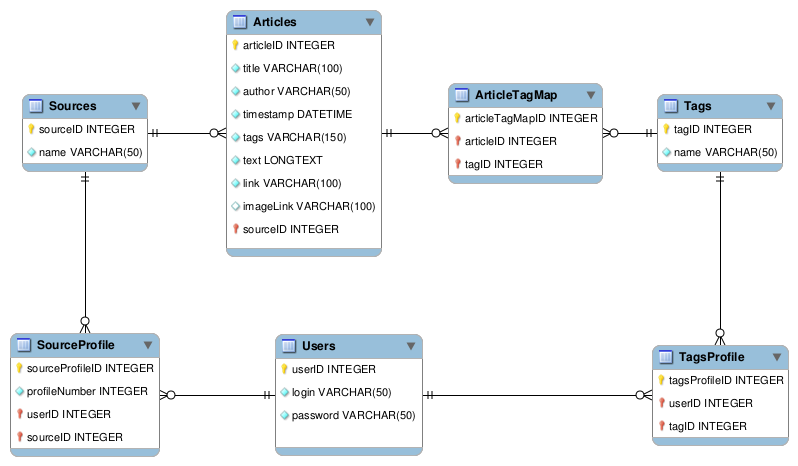
\includegraphics[scale=0.5]{obrazki/schemat_bd.png}
			\caption{Schemat bazy danych}
			\label{fig:db_schema}
		\end{figure}
	\begin{longtable}{ | C{5cm} | C{12cm} | @{}m{0pt}@{}}
		\caption{Opis bazy danych}
		\label{opis_bazy_danych}
		\endfirsthead % musi byc
		\multicolumn{3}{c}%
		{\tablename\ \thetable\ -- \textit{Kontynuacja}}\hfill \\
		\hline
		\textbf{Tabela} & \textbf{Opis} &\\[1cm]
		\hline
		\endhead
		% ostatnie krzaki to wysokosc wiersza
		\hline % ostatnia pusta kolumna to trik -> zle wyrownanie ostatniej kolumny
		\textbf{Tabela} & \textbf{Opis} &\\[1cm]
		\hline	
		Articles &
		Zawiera wszystkie sparsowane strony. (teraz kwestia ile je tam trzymać??) &\\[1cm] 
		\hline
		Tags &
		Zawiera wszystkie dostępne tagi. Dodanie nowego taga odbywa się automatycznie, gdy scraper podczas parsowania wykryje, że danego taga jeszcze nie ma w bazie. &\\[1.5cm]
		\hline
		ArticleTagMap &
		Łączy daną stronę z odpowiednim tagiem. &\\[1cm]
		\hline
		Sources &
		Zawiera wszystkie dostępne źródła, czyli strony internetowe, z których zbieramy dane. Dodanie odbywa się ręcznie. Administrator musi napisać moduł dla danej strony. &\\[1.5cm]
		\hline
		ArticleSourceMap &
		Łączy daną stronę z odpowiednią stroną z której pochodzi. &\\[1cm]
		\hline
		Users &
		Zawiera wszystkich użytkowników serwisu. &\\[1cm]
		\hline
		TagsProfile &
		Łączy użytkownika z tagami, które wybrał. &\\[1cm]
		\hline
		SourceProfile &
		Łączy użytkownika z źródłami danych, które wybrał. &\\[1cm]
		\hline
	\end{longtable}
	\section{Interesujące problemy i ich rozwiązania}
	
	\section{Opis stron internetowych, z których zbierane są informacje}
	\renewcommand\thesubsection{}
		\subsection{sekurak.pl}
		\begin{table}[H]
			\centering
			\caption{Parametry artykułów - sekurak.pl}
			\label{sekurak_parametry}
			\begin{tabular}{ | C{2cm} | C{4cm} | C{2cm} | C{2cm} | C{3cm} | C{2cm} | @{}m{0pt}@{}}
				\hline
				Tytuł & Data opublikowania & Tagi & Obrazek & Fragment tekstu & Link &\\[0.5cm]
				\hline
			\end{tabular}
		\end{table}

		\subsection{dobreprogramy.pl/Blog.html} 
		\begin{table}[H]
			\centering
			\caption{Parametry artykułów - dobreprogramy.pl}
			\label{dobreprogramy_parametry}
			\begin{tabular}{ | C{2cm} | C{4cm} | C{2cm} | C{2cm} | C{3cm} | C{2cm} | @{}m{0pt}@{}}
				\hline
				Tytuł & Data opublikowania & Tagi & Autor & Fragment tekstu & Link &\\[0.5cm]
				\hline
			\end{tabular}
		\end{table}
		\subsection{niebezpiecznik.pl} 
		\begin{table}[H]
			\centering
			\caption{Parametry artykułów - niebezpiecznik.pl}
			\label{niebezpiecznik_parametry}
			\begin{tabular}{ | C{1.5cm} | C{4cm} | C{1.5cm} | C{1.5cm} | C{1.5cm} | C{3cm} | C{1.5cm} | @{}m{0pt}@{}}
				\hline
				Tytuł & Data opublikowania & Tagi & Autor & Obrazek & Fragment tekstu & Link &\\[0.5cm]
				\hline
			\end{tabular}
		\end{table}
		\subsection{zaufanatrzeciastrona.pl} 
		\begin{table}[H]
			\centering
			\caption{Parametry artykułów - zaufanatrzeciastrona.pl}
			\label{z3s_parametry}
			\begin{tabular}{ | C{1.5cm} | C{4cm} | C{1.5cm} | C{1.5cm} | C{1.5cm} | C{3cm} | C{1.5cm} | @{}m{0pt}@{}}
				\hline
				Tytuł & Data opublikowania & Tagi & Autor & Obrazek & Fragment tekstu & Link &\\[0.5cm]
				\hline
			\end{tabular}
		\end{table}
		\subsection{wykop.pl} 
		\begin{table}[H]
			\centering
			\caption{Parametry artykułów - wykop.pl}
			\label{wykop_parametry}
			\begin{tabular}{ | C{1.5cm} | C{4cm} | C{1.5cm} | C{1.5cm} | C{1.5cm} | C{3cm} | C{1.5cm} | @{}m{0pt}@{}}
				\hline
				Tytuł & Data opublikowania & Tagi & Autor & Obrazek & Fragment tekstu & Link &\\[0.5cm]
				\hline
			\end{tabular}
		\end{table}
	\section{Instrukcja użytkowania aplikacji}
	
\end{document}
